% fig1_overview.pdf -- KWelfareBench pipeline schematic (TikZ).
% Compile: PATH=$HOME/.TinyTeX/bin/x86_64-linux:$PATH xelatex _make_fig1_overview.tex
% Then rename _make_fig1_overview.pdf -> fig1_overview.pdf
\documentclass[border=2pt,tikz]{standalone}
\usepackage[T1]{fontenc}
\usepackage{lmodern}    % Latin Modern (vector at every size; consistent with Fig 2/6)
\usepackage{tikz}
\usetikzlibrary{positioning,arrows.meta,fit,backgrounds,calc}

\begin{document}
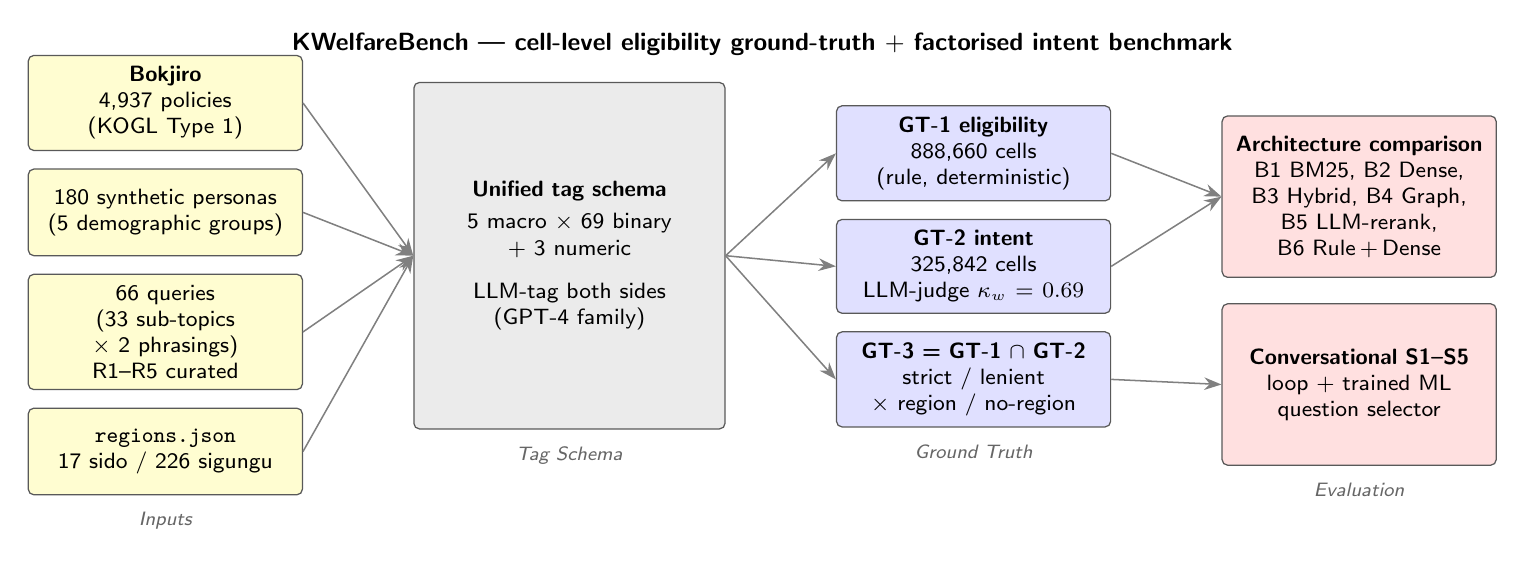
\begin{tikzpicture}[
  font=\sffamily,
  >={Stealth[length=2.2mm,width=1.6mm]},
  every node/.style={inner sep=2pt},
  basebox/.style={
    rectangle, rounded corners=2pt,
    draw=black!65, line width=0.45pt,
    align=center, text width=3.2cm,
    minimum height=1.10cm,
    inner sep=4pt,
    font=\sffamily\fontsize{7.8}{9.4}\selectfont,
  },
  hdr/.style={font=\sffamily\bfseries\fontsize{8.5}{10}\selectfont},
  inputbox/.style={basebox, fill=yellow!18},
  schemabox/.style={basebox, fill=black!8,
    text width=3.6cm, minimum height=4.4cm,
    inner sep=5pt,
    font=\sffamily\fontsize{7.8}{9.6}\selectfont,
  },
  gtbox/.style={basebox, fill=blue!12},
  evalbox/.style={basebox, fill=red!12,
    text width=3.2cm, minimum height=2.05cm,
    inner sep=4pt,
    font=\sffamily\fontsize{7.8}{9.4}\selectfont,
  },
  arr/.style={->, draw=black!50, line width=0.55pt},
]

%---------- column header positions (x in cm, top-down stacking) ----------
% column 1 (Inputs)
\node[inputbox] (in1) at (0.0, 0.0)
  {\textbf{Bokjiro}\\4{,}937 policies\\(KOGL Type 1)};
\node[inputbox, below=0.22cm of in1] (in2)
  {180 synthetic personas\\(5 demographic groups)};
\node[inputbox, below=0.22cm of in2] (in3)
  {66 queries\\(33 sub-topics $\times$ 2 phrasings)\\R1--R5 curated};
\node[inputbox, below=0.22cm of in3] (in4)
  {\texttt{regions.json}\\17 sido / 226 sigungu};

% column 2 (Schema) -- centered vertically against col1
\node[schemabox, right=1.4cm of in2.east, anchor=west, yshift=-0.55cm] (sch)
  {\textbf{Unified tag schema}\\[2pt]
   5 macro $\times$ 69 binary\\
   $+$ 3 numeric\\[6pt]
   LLM-tag both sides\\
   (GPT-4 family)};

% column 3 (GT)
\node[gtbox, right=1.4cm of sch.east, anchor=west, yshift=1.30cm] (gt1)
  {\textbf{GT-1 eligibility}\\888{,}660 cells\\(rule, deterministic)};
\node[gtbox, below=0.22cm of gt1] (gt2)
  {\textbf{GT-2 intent}\\325{,}842 cells\\LLM-judge $\kappa_w = 0.69$};
\node[gtbox, below=0.22cm of gt2] (gt3)
  {\textbf{GT-3 = GT-1 $\cap$ GT-2}\\strict / lenient\\$\times$ region / no-region};

% column 4 (Eval)
\node[evalbox, right=1.4cm of gt1.east, anchor=west, yshift=-0.55cm] (ev1)
  {\textbf{Architecture comparison}\\
   B1 BM25, B2 Dense,\\
   B3 Hybrid, B4 Graph,\\
   B5 LLM-rerank,\\
   B6 Rule\,+\,Dense};
\node[evalbox, below=0.32cm of ev1] (ev2)
  {\textbf{Conversational S1--S5}\\
   loop $+$ trained ML\\
   question selector};

%---------- arrows ----------
\foreach \src in {in1,in2,in3,in4}{
  \draw[arr] (\src.east) -- (sch.west);
}
\draw[arr] (sch.east) -- (gt1.west);
\draw[arr] (sch.east) -- (gt2.west);
\draw[arr] (sch.east) -- (gt3.west);
\draw[arr] (gt1.east) -- (ev1.west);
\draw[arr] (gt2.east) -- (ev1.west);
\draw[arr] (gt3.east) -- (ev2.west);

%---------- title strip ----------
\node[anchor=south, font=\sffamily\bfseries\fontsize{9.5}{11}\selectfont]
  at ($(in1.north)!0.5!(ev1.north) + (0,0.30)$)
  {KWelfareBench --- cell-level eligibility ground-truth $+$ factorised intent benchmark};

%---------- column captions (small, gray) ----------
\node[anchor=north, font=\sffamily\itshape\fontsize{7.2}{8}\selectfont, text=black!60]
  at ($(in4.south) + (0,-0.14)$) {Inputs};
\node[anchor=north, font=\sffamily\itshape\fontsize{7.2}{8}\selectfont, text=black!60]
  at ($(sch.south) + (0,-0.14)$) {Tag Schema};
\node[anchor=north, font=\sffamily\itshape\fontsize{7.2}{8}\selectfont, text=black!60]
  at ($(gt3.south) + (0,-0.14)$) {Ground Truth};
\node[anchor=north, font=\sffamily\itshape\fontsize{7.2}{8}\selectfont, text=black!60]
  at ($(ev2.south) + (0,-0.14)$) {Evaluation};

\end{tikzpicture}
\end{document}
